\documentclass{article}
\usepackage{listings}
\usepackage{xcolor}

\definecolor{codegreen}{rgb}{0,0.6,0}
\definecolor{codegray}{rgb}{0.5,0.5,0.5}
\definecolor{codepurple}{rgb}{0.58,0,0.82}
\definecolor{backcolour}{rgb}{0.95,0.95,0.92}

\lstdefinestyle{mystyle}{
    float=tp,
    floatplacement=tbp,
    backgroundcolor=\color{backcolour},   
    commentstyle=\color{codegreen},
    keywordstyle=\color{magenta},
    numberstyle=\tiny\color{codegray},
    stringstyle=\color{codepurple},
    basicstyle=\ttfamily\footnotesize,
    breakatwhitespace=false,         
    breaklines=true,                 
    captionpos=b,                    
    keepspaces=true,                 
    numbers=left,                    
    numbersep=5pt,                  
    showspaces=false,                
    showstringspaces=false,
    showtabs=false,                  
    tabsize=2
}

\lstset{style=mystyle}
\usepackage{graphicx} % Required for inserting images
\usepackage[style=ieee]{biblatex}
\addbibresource{ref.bib}
\usepackage[letterpaper]{geometry}
% \usepackage[letterpaper, total={7in, 9in}]{geometry}
\renewcommand*{\bibfont}{\footnotesize}

\begin{document}
\title{3D2Mol: Converting Molecular Model Images to Digital Representations to Improve Student Understanding}


\author{Wenqi Marshall Guo\\
Department of CMPS\\
University of British Columbia\\
Kelowna, BC\\
wg25r@student.ubc.ca 
\and
Mohamed Shehata\\
Department of CMPS\\
University of British Columbia\\
Kelowna, BC\\
mohamed.sami.shehata@ubc.ca
}

\maketitle


\begin{abstract}
Molecular models 
\end{abstract}


\section{Introduction}
Molecular models are helpful tools in chemistry education as they provide an intuitive way for students to understand the 3D structure compared to 2D molecular structure representation. These models can also assist students with 3D mental operations. 
% Although virtual models could be as effective as concrete models, concrete should be available to students at least at the beginning of the study of new concepts and ideas, as humans sometimes rely on concrete objects.\autocite{savec_evaluating_2005} 
A study \autocite{savec_evaluating_2005} found that virtual models could have the same effectiveness as concrete models, students should have access to concrete models at least at the beginning of the study because sometimes humans rely on concrete objects.  
However, digital model representation has the benefit that allowing students to look up more information about the molecule such as the IUPAC name and the boiling point. Students can also modify the molecule and observe how it will affect the molecular properties. Thus, it will be beneficial if students can convert concrete molecular models to digital representations. 

Although there are models that can convert 2D molecular structure representations to corresponding digital representations \autocite{swinocsr}\autocite{decimer}\autocite{chempix}, to the best of our knowledge, there is not a model for 3D molecular models. It will be beneficial to chemical education to close this gap between 3D molecular models and digital representations. 
Our contribution to this paper can be summarised as:
\begin{itemize}
\item We have constructed two datasets: one computer-rendered 3D molecular model and another consisting of real-world 3D molecular models.
\item We trained a model on top of these two datasets that is capable of converting images of concrete molecular models into their respective SMILES notations. 
\item We applied a method based on multi-image input and beam search to increase the accuracy of the output.
\item We proposed for the model to re-evoluet its own output to select more clbarated result, self negative
% can we use this for seg? review the segmented images
% \item We applied a multi-image input method allowing users to capture multiple images of the molecular model to increase the accuracy of the output.
\end{itemize}

\section{Related Work}
To the best of our knowledge, there is no prior model that can convert a 3D molecular set photo into its digital structure representation. However, there are some models for 2D structure formulas. The two most recent ones are SwinOCSR\autocite{swinocsr} and DECIMER.ai\footnote{The name DECIMER has been used by the same team for both the dataset and two versions of the mode, here we are refreshing the model published in 2023.}\autocite{decimer}. These two models are very similar in architecture consisting of an image encoder and a transformer.

% The decoder used in 
\subsection{DECIMER.ai}
In DECIMER.ai, the encoder is an EfficientNet-V2-M. EfficientNet is a type of convolutional neural network (CNN) with MBConv \autocite{tan_efficientnet:_2020} (a modified version of the inverted bottleneck from \autocite{mobilenet}) and Fused-MBConv \autocite{suyog_efficientnet-edgetpu:_2019} developed by training-aware neural architecture search (NAS). \autocite{swin_tran} \autocite{effv2} MBConvs have 1$\times$1 point-wise and 3$\times$3 depth-wise convolutional layers, which can yield better parameters and computational efficiency. \autocite{mobilenet} \autocite{effv2} However, they cannot fully utilize modern hardware accelerators. In Efficient-Net-V2, they proposed using regular 3x3 convolutional layers (Fused-MBConvs) to replace MBConvs for the early stages of the network. This results in better training time with small overheads of parameters and FLOPs. In an MBConv block used in Efficient-Net-V2, the image is first passed through a 1x1 convolutional layer to increase its channel numbers, then a squeeze and excitation (SE) block is used \autocite{hu_squeeze-and-excitation_2019}\autocite{tan_efficientnet:_2020}. SE blocks are shown to increase the performance of CNNs with slight computational overhead. \autocite{hu_squeeze-and-excitation_2019}. The SE block is followed by a depthwise 3x3 convolution and a 1x1 convolution, the latter decreases the channel counts to the same as input. In a Fused-MBConv, however, the depthwise convolution and the 1x1 convolution are replaced by a 3x3 convolution. \autocite{effv2} \autocite{mobilenet}

The decoder in DECIMER.ai is a transformer model based on \autocite{attention_is_all_you_need}. It has four transformer encoder blocks and four transformer decoder blocks with right parallel attention heads. \autocite{decimer} The encoder of the transformer utilizes a multi-head self-attention block and an MLP (multilayer perceptron) to replace previous recurrent neural or convolutional layers. The decoder of the Transformer is auto-regressive, meaning the decoder of the model takes in the already generated sequence and predicts the next token. The generated sequence will be processed by a masked multi-head self-attention. The mask will prevent the model from attending tokens after $t$ when generating the $t$-th sequence. Then a cross-attention layer is applied that connects the input sequence and the generated sequence by using the output of the encoder as keys and values and output from the masked self-attention as the query. Then the output of the cross-attention is followed by an MLP layer. The encoder and decoder blocks are repeated for $N$ (In DECIMER.ai $N=4$) times each. After the last decoder block, the output goes through a linear and a softmax layer before output. Since attention does not consider position information, position encoding is added to the sequence for both input and generated sequences. The full transformer also uses residual connection across all the attention and MLP layers. After the addition of the residual connection, a layer normalization is used. A detailed architecture of the Transformer can be found in the original paper \autocite{attention_is_all_you_need}. 

Although DeepSMILES \autocite{oboyle_deepsmiles:_2018} has been proposed for machine learning models to generate more valid identifies, their previous work \autocite{rajan_performance_2022} has shown that SMILES actually lead to the most accurate identifiers. Thus, they used SMILES instead of DeepSMILES in DECIMER.ai. \autocite{decimer}  

%how it trained on real data and handwritten 
\subsection{SwinOCSR}
In SwinOCSR, the encoder (they referred to as "backbone" in their paper) is built on the Swin Transformer. The image is cut into patches with each path having a size of $4 \times 4$ pixels. Then each patch is flattened into and treated as a token which is a 48-dim vector. Then a linear projection layer is applied and each token is into a 192-dim space. 
Then 4 Swin-Transformer (Shifted Window Transformer) \autocite{swin_tran} blocks are used. Each swim transformer block contains two regular transformer modules. In the first transformer module, Window Mutli-head Self Attention (W-MSA) is performed within each window, which is a group of neighbouring tokens. In the second transformer module, the Shifted Window Mutli-head Self Attention (SW-MSA) is performed on a shift-ed window. The W-MSA allows the model to capture the local relationship in the image, and the SW-MSA introduced a cross-window connection while maintaining efficiency. After each block, a patch merging operation is performed such that neighbouring patches are merged and the tokens are contacted. \autocite{swin_tran} The decoder of SwinOCSR is very similar to the decoder in DECIMER.ai, which is also a transformer encoder-decoder pair but with 6 blocks of encoders and 6 blocks of decoders. In additition, SwinOCSR uses focal loss \autocite{lin_focal_2018} instead of normal cross entropy loss due to the inbalance of the tokens distribution. \cite{swinocsr}

% Moved down here To this point, we get a tensor of $\frac{H}{4} \times \frac{W}{4} \times 48$ where $W$ and $H$ are the width and height of the original image. 
% Before the tensor ($H_i \times W_i \times C_i$) gets passed to the next Swin Transformer block, a patch merging operation is performed to capture hierarchical information. During path merging, neighbouring $2 \times 2$ patches are merged and the tokens are concatenated. This results in $\frac{1}{4}$ of the number of patches and each $4C_i$ feature for each token. Then the dimensions of each token are reduced to $2C_i$. In SwinOCSR, 4 Swin Transformer blocks are used; the last Swin Transformer block outputs a tensor with shape $\frac{H}{32} \times \frac{H}{32} \times 1536$. This tensor is flattened across the spatial axes and projects the last axis into 256 dimensions. 

%how it trained using a special loss function  
% deepsmiles


% \subsection{Re-evoluate the Results After Generation}



\section{Method}
In addition, DECIMER.ai also attempted to recognize hand-drawn structures by finetuning the model with a dataset that has augmented data that makes structures look hand-drawn. \autocite{decimer} We adapted this two-stage training process in our project. The model is first trained on a synthetic (3D rendered) dataset and then finetuned on a real-world collected dataset to reduce the amount of real-world data that needs to be collected as they are expensive.  
\subsection{Synthetic Dataset}
\begin{figure}
    \centering
    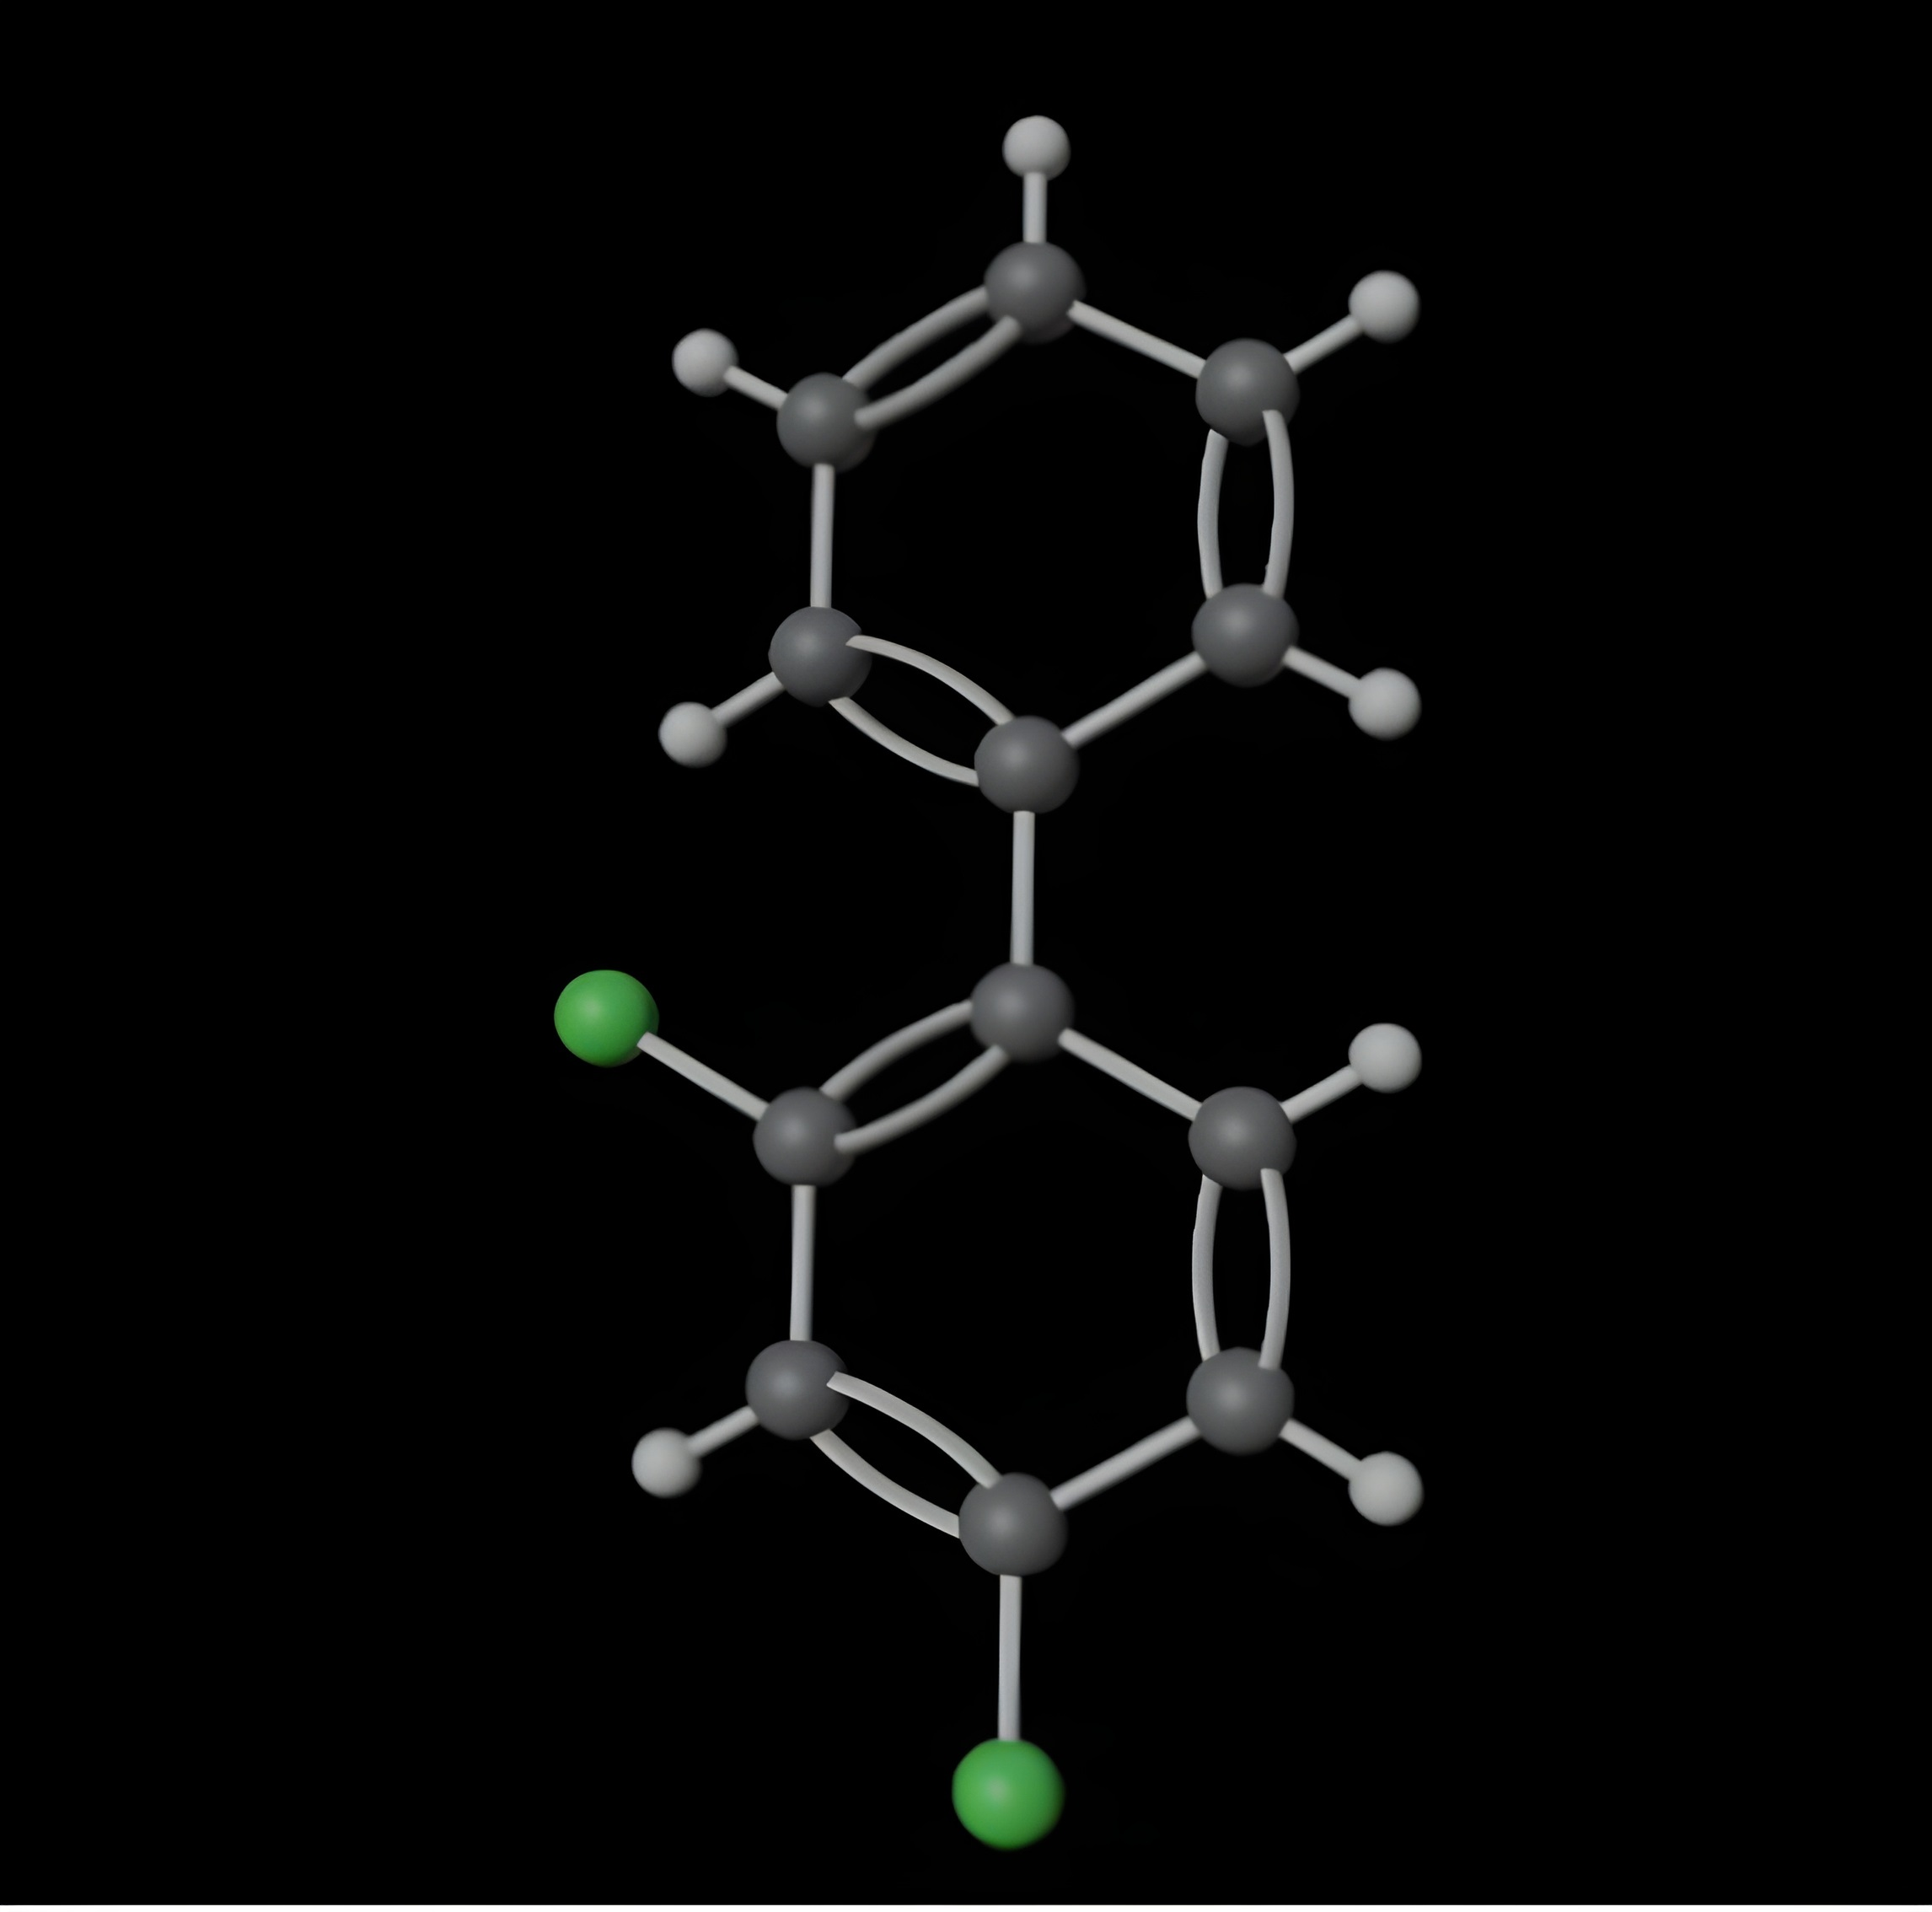
\includegraphics[width=0.3\textwidth]{generated}
    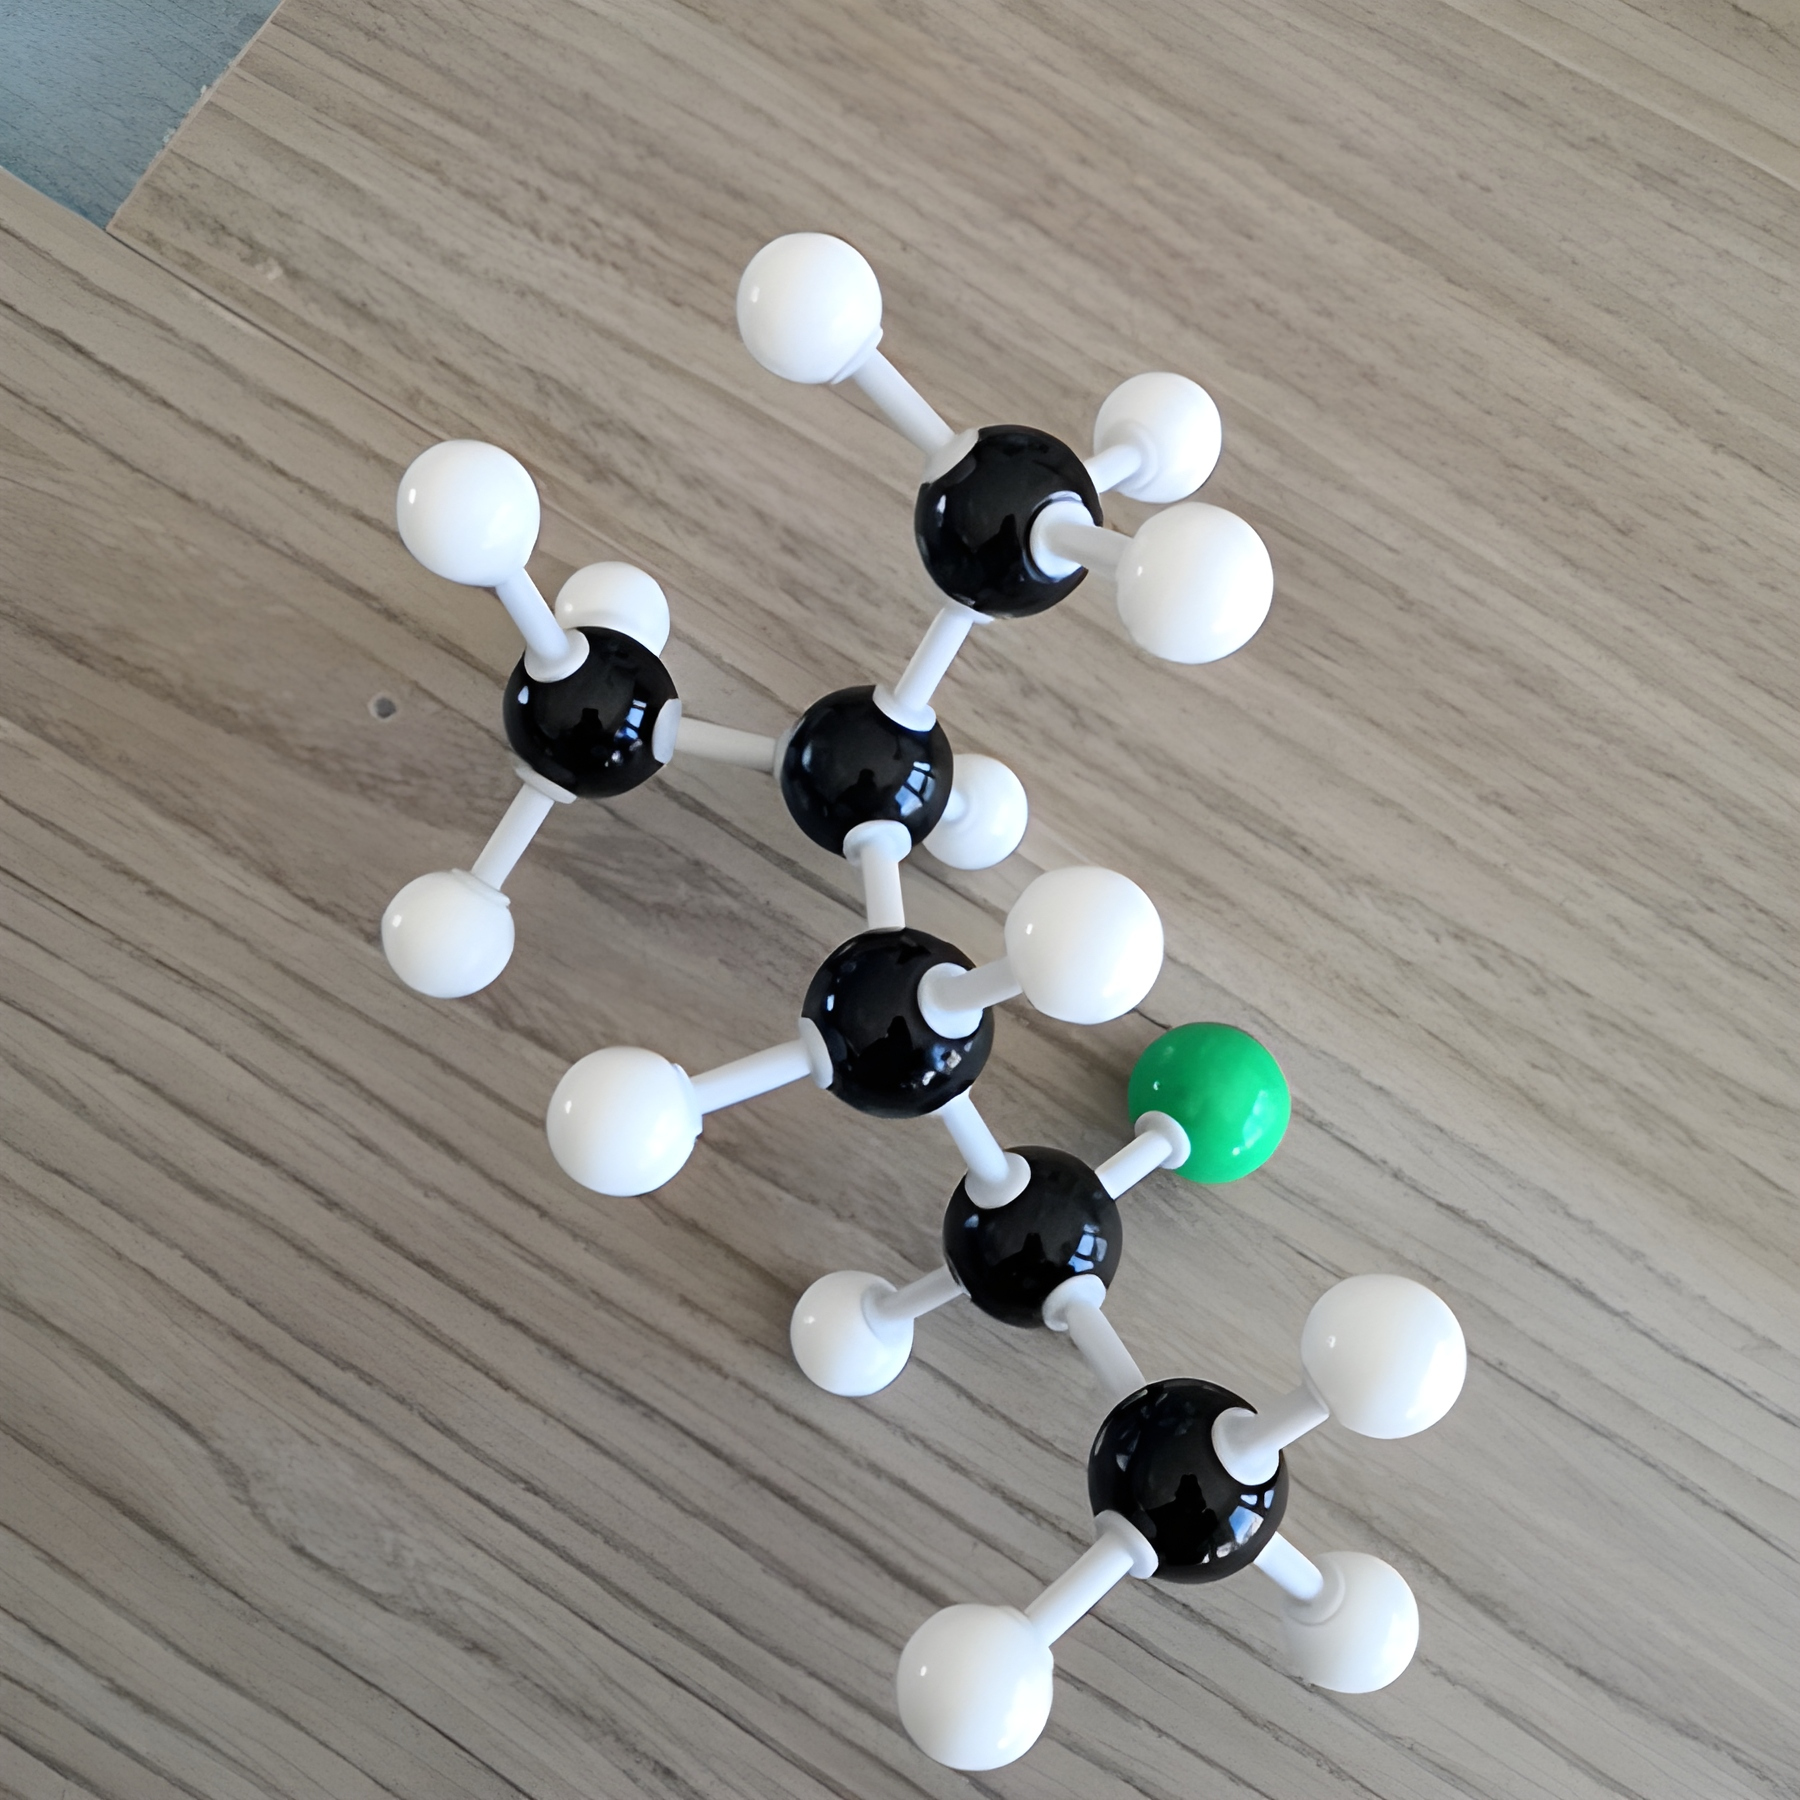
\includegraphics[width=0.3\textwidth]{cap}
    \caption{A rendered image of 2,4-Dichlorobiphenyl and real captured image of 2-Chloro-4-methylpentane}
    \label{fig:example}
\end{figure}

We downloaded a set of compounds from PubChem \autocite{kim_pubchem_2023}, and then these compounds were filtered based on heavy atoms and molecular weights and only contained elements of C, O, S, H, N, Cl, Br, F, and P. Because of the complex 3D nature of molecules, there could be occlusions between atoms and bonds, where important information is hidden in the image. Although there are methods to avoid `occlusions by some spatial algorithm or human selection, we decided to remove 3D spatial information in the pretraining stage. Thus, we downloaded the 2D coordinate from PubChem instead of 3D.  
% filtered such that the compounds have at most X atoms \footnote{We did not directly limit the number of atoms on PubChem queries: we limited the number of heavy atoms and molecular weight, which yielded in the limitation of atoms.} 
After filtering, there are 79,369 compounds in the dataset. The pre-train training and validation sets are separated by image IDs. We created a Blender Python Script to render these compounds into 3D molecular images. OpenAI ChatGPT was used to write the building blocks (API Wrapper) and some logic of the script. The colour of each atom follows the CPK colouring convention and was according to a couple of online sources and 3D molecular models on the market. For each molecule, we rendered 4 different images at different angles. Detailed render process can be found in our GitHub repository. 
% self negative example: gan
% Rendered from 2D information ....

%redo
We observed that image size will affect the convergence speed of the model and the traditional image size used for classification ($224\times224$) is not enough for our task; thus, we used an image size of $400\times400$. 
\subsection{Real-World Dataset}
We created a mobile application using React.js for data collection. To increase the efficiency of data collection, we group similar models using the GPT: a list of the names of the molecules is given to the GPT via the OpenAI API and asked to group similar molecules together. Users can build either the given molecules or another molecule they choose. Volunteers are recruited to collect these images of molecular models. Because some of the molecular model kits we used do not have sulfur, we excluded all molecules with sulfur. After collecting, we observed some low-quality data such as images with obstruction between atoms, motion blur, etc. Thus, we made another application allowing volunteers to go through all the images and decide if they will be kept or discarded.

We separated the training set and validation set by SMILES strings (i.e. different images of the same molecule will not appear in both validation and training set. Since we ignored isotopes here, molecules with different IDs might have the same SMILES) The validation set is randomly selected such that it has 20 molecules and 214 images total. 

The images are collected on clear backgrounds, and for each molecule images with different camera angles are captured. In total, we have a total of X images of Y molecules. 

Figure \ref{fig:example} shows an example of rendered and real images. These images are images from the dataset after super-resolution for better visualization. 
\subsection{Machine Learning Model} 
\subsubsection{Basic Model}
\begin{figure}
    \centering
    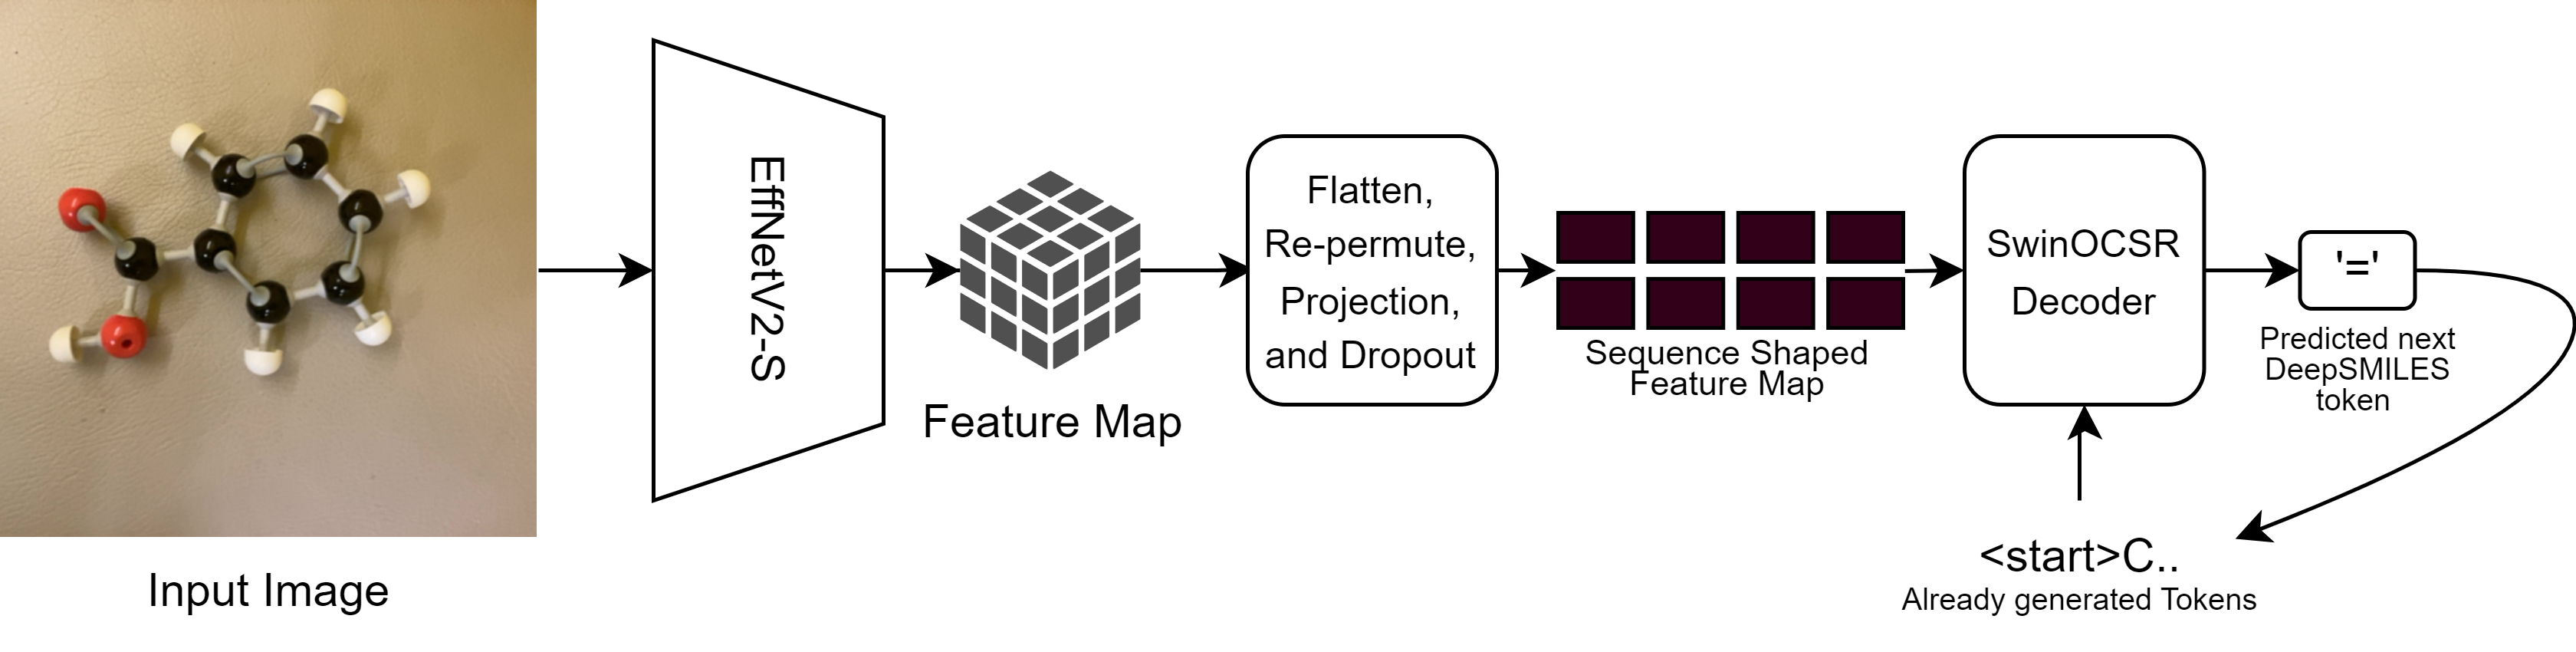
\includegraphics[width=0.9\textwidth]{arch}
    \caption{Model Architecture}
    \label{fig:arch}
\end{figure}
Our model architecture is shown in Fig \ref{fig:arch} and is very similar to the ones used in DECIMER.ai \autocite{decimer} and SwinOCSR \autocite{swinocsr}. The encoder we used is the EfficientNet-V2-S \autocite{effv2} from torchvision \autocite{torchvision2016} with internal parameters that are trained on ImageNet-1k \autocite{imagenet}. We extracted all the convolution layers from the EffcientNet-V2-S to get a feature map with size $1280\times13\times13$  for each batch. This feature map is then flattened into 2D shape $1280\times169$, re-permuted to sequence-like shape $169\times1280$, projected to 256-dimension to match the input shape of SwinOCSR decoder, and passed through a dropout layer. The tensor is then fed into our decoder. which is adapted from SwinOCSR \autocite{swinocsr}. 

\subsection{Beam search and Multi-image input}
Beam search is a way to increase the accuracy of autoregressive models. \autocite{yang_breaking_2018} \autocite{zhang_beam_2024}. Beam search can also provide users with multiple candidate answers to choose from, similar to the top-$n$ in image classification. However, one issue with beam search is that it will favour shorter sequences as a sub-sequence will always have a higher probability than its parent sequence. \autocite{yang_breaking_2018} \autocite{zhang_beam_2024} There are multiple methods to solve this issue, some are mentioned in \autocite{yang_breaking_2018} and \autocite{zhang_beam_2024}. In this paper, we use a simple method mentioned in \autocite{zhang_beam_2024} where we multiple  $\frac{1}{L^\alpha}$ to the log probability where $L$ is the length of the sequence. This will make the log probability of a long sequence higher (since the log probability is negative). 
% In this project, we set \(\alpha=0.75\) as suggested in \autocite{zhang_beam_2024}.

Additionally, we also hypothesize that multiple image inputs will increase the accuracy of the model. This has been shown in previous research \autocite{sun_multi-input_2017}, in which the authors use ``early fusion" method where feature maps from 3 different images are concatenated on the channel axis in the early stage of the network. However, this method requires modification of the backbone network and the number of images in this method is fixed. Instead, our method passes individual images through the entire network (including the EfficientNet-V2-S and SwinOCSR decoder) and averages the softmax distribution of tokens.  


\subsection{Improve Accuracy By Self-Reflection}
%should i put this in related works
It has been shown that in Large Language Models (LLMs), it might be hard for the model to output useful and safe information, but it is easy for the model to find it after re-evaluating it. \autocite{bai_constitutional_2022} Similar ideas have been shown in some image-text generative models such as DALL-E \autocite{ramesh_zero-shot_2021} and CLIPasso \autocite{vinker_clipasso_2022} where another model (in these two cases, CLIP \autocite{radford_learning_2021}) to evaluate multiple output of the generative model and select the best output in the generated. There are also some image-text matching evolution metrics being proposed such as CLIPScore \autocite{hessel_clipscore:_2022} and image-text matching loss \autocite{xu_attngan:_2017} to evaluate the similarity between text and image. 

However, CLIP is a contrastive learning model: for a given number of image-text pairs, feature of each image and text is extracted by its corresponding encoder, then in the embedding space, it is treated as a multi-class classification problem to match each image with corresponding text. \cite{radford_learning_2021} Thus, it usually requires a large number of negative samples (32,768 in \autocite{radford_learning_2021}) in the batch for the model to learn useful information. \autocite{he_momentum_2020} Although there are models like Momentum Contrast  (MoCo) \autocite{he_momentum_2020} to build a large negative sample queue using a smaller batch size by momentum for pure image tasks, it is hard to use such strategy for multi-modality tasks involving both text and images without adding complexity to the model or training pipeline. 

Image-text matching loss (being used in many multi modality models, such as \autocite{li_align_2021} \autocite{liao_evaluation_2023}\autocite{xu_attngan:_2017}), on the other hand, dose not treat this problem as a multi-class classification problem but a binary classification problem. That is, for each pair of image and text, the model need to determine if it is a matched pair. This method dose not require a large batch size and can be trained on a single GPU. The models we used involving a transformer decoder, unlike \autocite{li_align_2021} and \autocite{kim_vilt:_2021} which use the transformer encoder, we put the feature extraction token at the end of the sequence, like in Generative Pre-trained Transformer-1 (GPT-1) \autocite{alec_improving_nodate}. Specifically, when the model output the \verb|<end>| token, this will be appended to the \textit{generated sequence} same as other tokens, and when the model got this token as input, the output of the last layer of the transformer will not be projected to predict tokens but projected to do a binary classification for image-text matching. This process can be found in Figure \ref{fig:itm}.

\begin{figure}
    \centering
    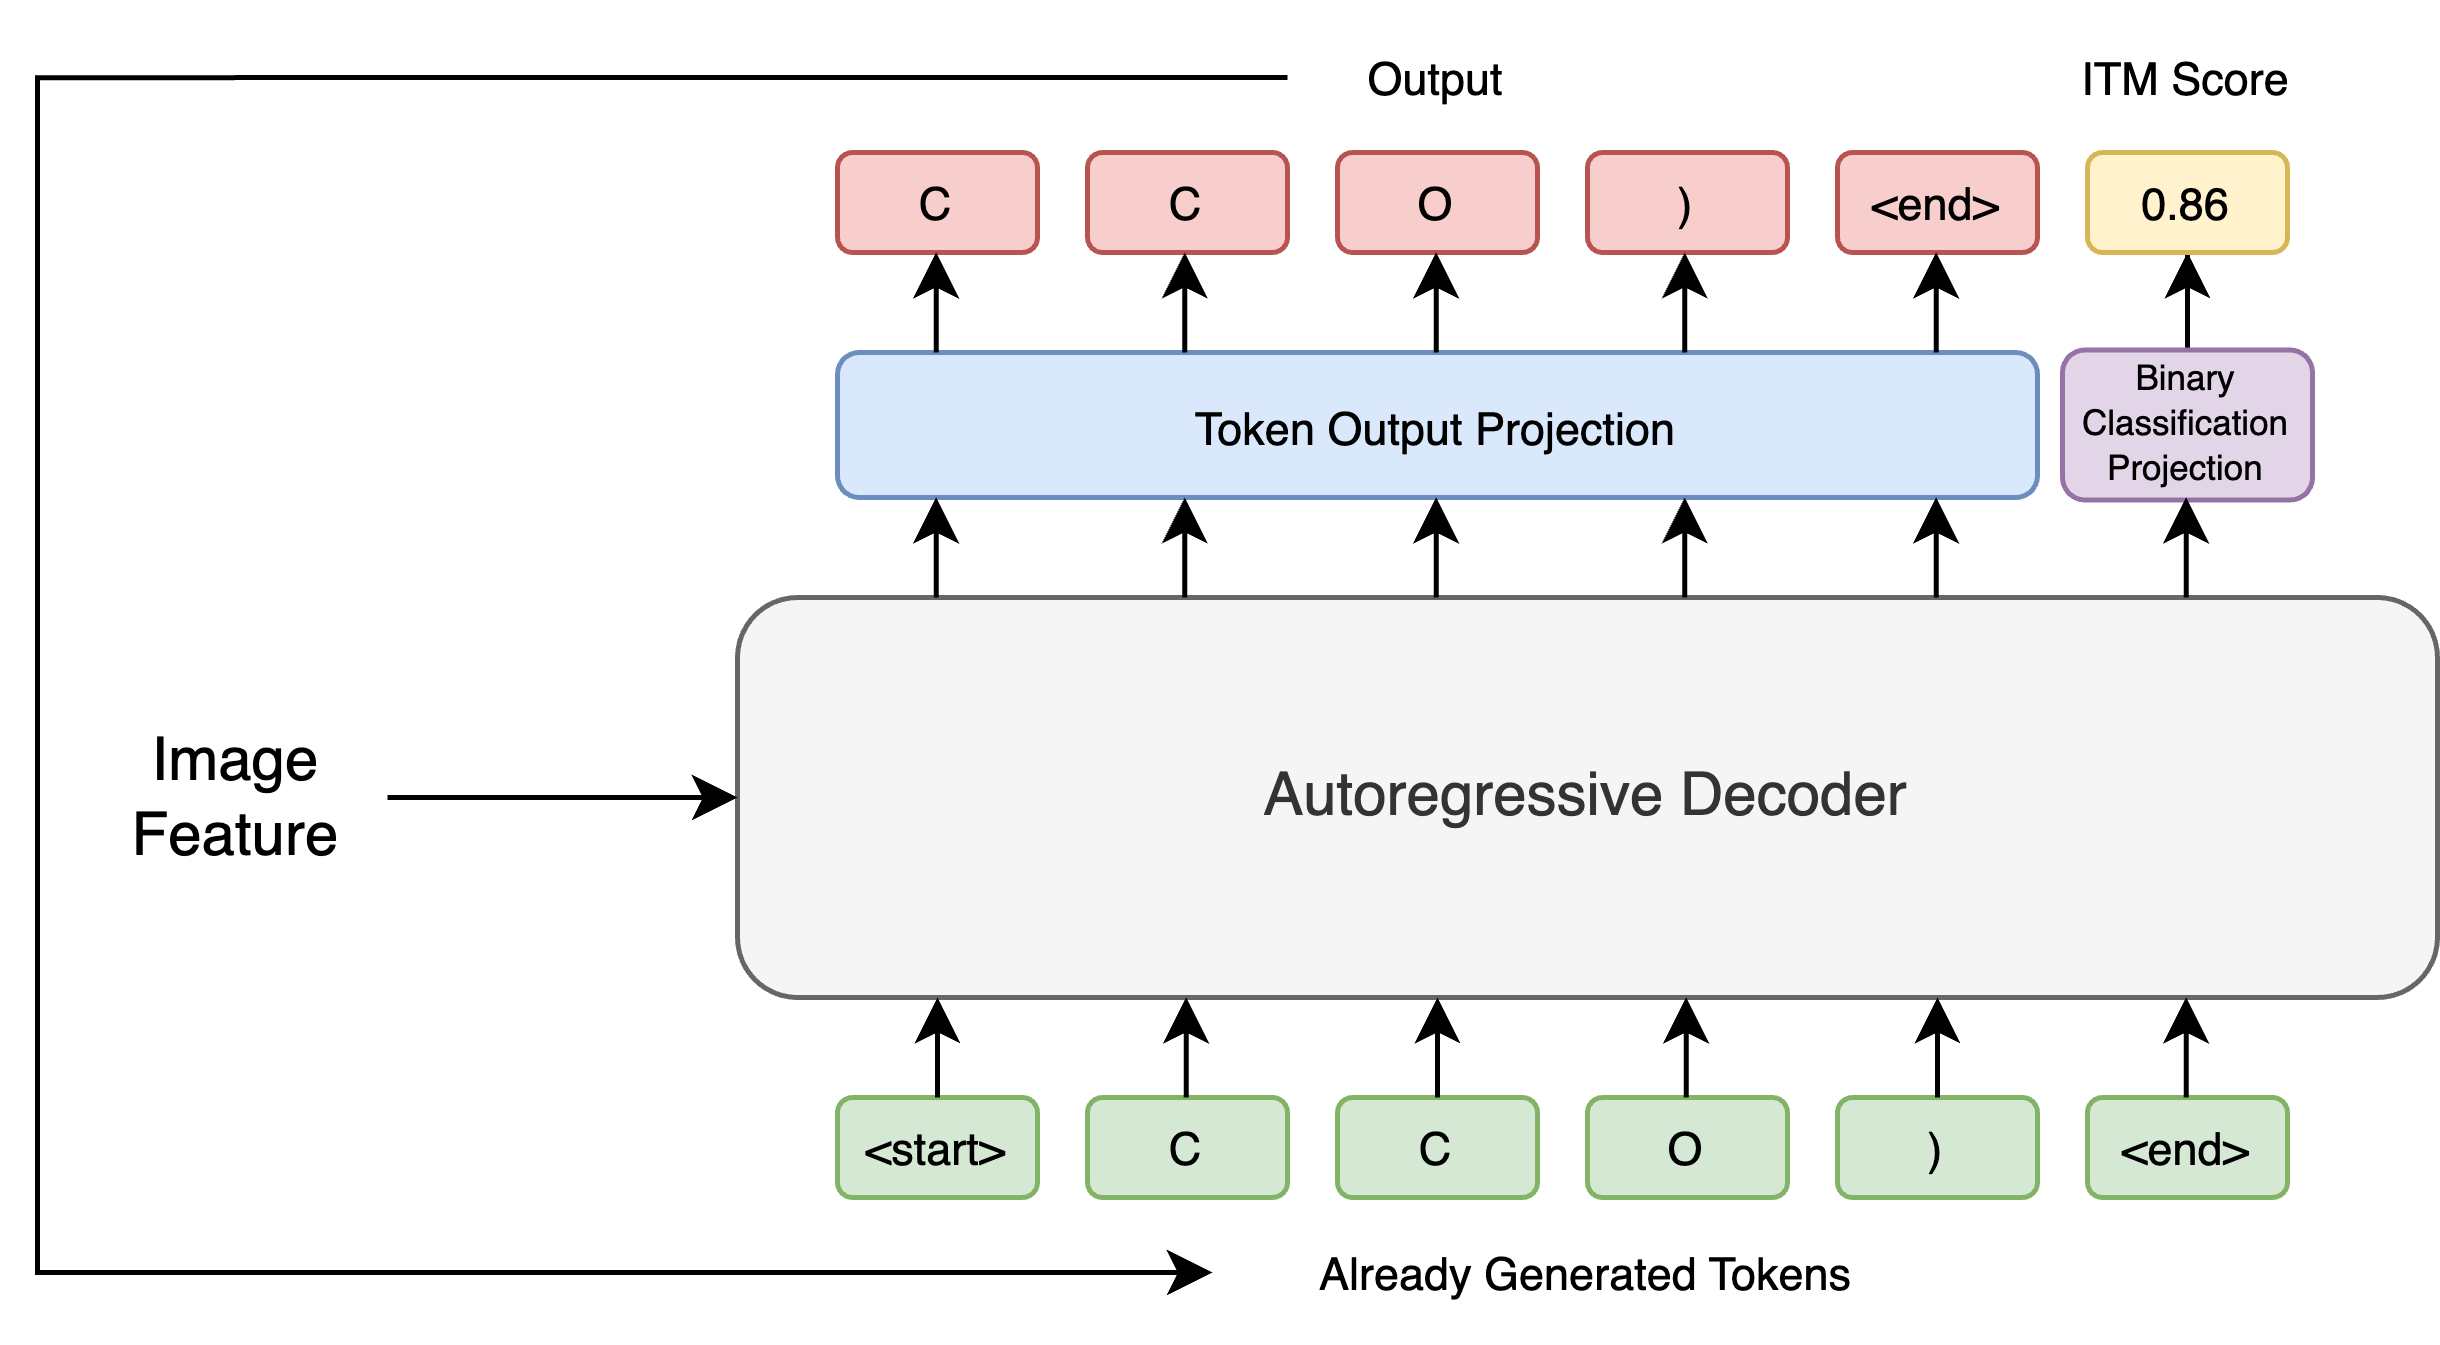
\includegraphics[width=0.5\linewidth]{itm.drawio.png}
    \caption{Model With Image-Text Matching}
    \label{fig:itm}
\end{figure}
Since the purpose of the ITM score is to find the best sequence in multiple model-generated sequences, it will be beneficial for use model's mistake as negative examples in ITM training. To achieve this, we maintain a dictionary with the values are queues of recent wrong model-generated output and keys are the correct answer. At the begining, the queue is initialized with random DeepSMILES strings in the training (we did not exclude the correct answer because it will add computational overhead and the chance of selecting the correct answer in it is very low) set and progressively being replaced by model output. By using this method, model can learn from its own mistakes. This task will also getting progressively more difficult because as the model trains, its output will get more simlar to the correct answer even when it is wrong. This pseudocode can be found in Listing \ref{selfnagative}, detail such as translating between tokenized sequences and DeepSMILES, remvobing special tokens, reshaping, are not included.   

\begin{minipage}{\linewidth}

\begin{lstlisting}[language=Python, caption=Training Process Pseudocode, label=selfnagative]
mistakes = {correct:random.choices(SMILES, k=3) for correct in SMILES}

# training loop
for img, text_in, text_out in dataloader():
    # text_in is <start>SMILES<end>, text_out is SMILES<end>
    optimizer.zero_grad()
    outputs = model(image, text_in, predict = True)[:,:-1,:]
    loss = focal_loss(outputs, text_out)
    loss.backward()
    optimizer.step()
    
    if outputs != text_out:
        mistakes[text_out].append(outputs)
        mistakes[text_out].pop(0)
    
    label = [random()<0.5 for _ in range(BATCH_SIZE)]
    text_in = [text_out[i] if j else random.choice(mistakes[text_out[i]]) for i, j in enumerate(label)]
    optimizer.zero_grad()
    # predict = False for binary classification 
    outputs = model(image, text_in, predict = False)
    # * 1.2 to give ITM loss more weight
    loss = binary_cross_entropy_with_logits(outputs, label) * 1.2 
    loss.backward()
    optimizer.step()
\end{lstlisting}
\end{minipage}
    % for i in range(BATCH_SIZE):
    %     corr = text_out[i]
    %     if random.random()<0.5:
    %         text_in.append(corr)
    %         label.append(1)
    %     else:
    %         text_in.append(random.choice(mistakes[corr]))
    %         label.append(0)
\subsection{Experiment}

Since we have a small dataset for fine-tuning, we applied many random online data augmentation during the training process: random rotation, random flipping, random cropping,  and random colour jitter (including RGB channels and brightness). 

We train our model on the synthetic dataset with AdamW \autocite{adamw} and an exponential learning rate scheduler. We then fine-tune our model on the real-world dataset. With the fixed validation set, we did a hyperparameter search using both Weight and Bias \autocite{wandb} and manual tuning to select models with the highest validation token-level accuracy.  
% Similar to the pretraining, the decoder is frozen. 
Additionally, we also freeze the projection layer between the encoder and reladecoder and the last 2 blocks of encoder EfficientNet-V2-S since the input of the decoder is in the same domain for pre-training and finetuning. This could also decrease the number of trainable parameters to avoid overfitting. 
After training, we tested the model on a dataset between validation and testing. This dataset is not used in finetuning the hyperparameters but is used to test after hyperparameter tuning. However, it is not the final testing set. If the model performance is not ideal on this dataset, we returned the hyperparameters. This intermedia dataset could be used multiple times and will be merged into the validation set at the end and the model will be tested on a real dataset.
\section{Results and Discussions} 
There are also a few hyperparameters in inference that we need to consider: the softmax temperature ($t$), beam size ($n$), $\alpha$ in the beam search penalty for short sequences, and number of input images ($N$). We used Weight and Bias \cite{wandb} to do a random sweep with on these hyperparameters and selected the hyperparameter set with the highest score, which is defined in Equation \ref{score} where $P_{1}$ and $P_{n}$ are top-1 and top-$beam$ accuracy. We extended our validation set with some more molecules, this dataset is also filtered to remove images with occlusion and bad lighting. However, we kept some images that could be out of the domain for the model (poor lighting but atoms are still visible, and overly simplified molecule: methane) to avoid biased results from cherry-picking the data. For each molecule, take $k$ samples where $k$ is the number of images for that molecule in the dataset. For each sample, we randomly select $N$ images from the dataset without replacement. 


\begin{equation}
S = P_{1} + 0.9P_{n}
\label{score}
\end{equation}

\begin{table}[]
    \centering
    \begin{tabular}{c|cc}
      $beam$ & Top-1 Accuracy & Top-$beam$ Accuracy \\ \hline
      1 & 71.9 ± 5.8 & 71.9 ± 5.8 \\ 2 & 72.3 ± 5.8 & 79.8 ± 5.3 \\ 3 & 71.5 ± 5.8 & 84.6 ± 4.9 \\ 4 & 71.2 ± 5.8 & 86.9 ± 4.6 \\ 5 & 71.5 ± 5.8 & 87.3 ± 4.6
    \end{tabular}
    \caption{}
    \label{tab:my_label}
\end{table}

Since the above validation set is manually filtered and is used to finetune hyperparameters, it might not be a fair demonstration of our model's capacity Thus, we also tested the model capacity with the hyperparameter found on the validation set on a separately collected testing dataset. And the result of the testing dataset 
% I am not sure what to do here, sweep on test? Do not want to do so: no testing data. alex did not gave it to me. Also i need to find hyperparameter, should i compare it? zhihu said should be on validation 

compare the accuracy of different types of molecules
% compare with hand written OCSR 
% Since to the best of our knowledge, there is no pervious work targeting the same topic, we do not have any benchmark to compare to. However, the DECIMER.ai 
\section{Conclusion}
\section{Demo}
We deployed the model on our server \footnote{\url{http://file.weasoft.com:8888}} with a frontend and open source our model on github\footnote{\url{https://github.com/weathon/3d2smile}}. 
\section{Limation and Future Work}
In this project, we did not attempt to recognize stereochemical information such as chirality and E/Z structure. However, these are important concepts for students to understand and being able to show these is one of the key characteristics and benefits of 3D models. 
Our real-world dataset is limited by time and budget, a larger dataset could increase the accuracy and robustness of the model. 
This project only focused on the technical side of the problem and did not test how well this application would be in classroom settings, further chemical education studies are needed to determine its effectiveness in education. 
Traditional molecular models have some limitations, such as they might be misleading and let students think energy is needed to create bonds when they are not \autocite{snatoms}. Train a machine learning model on alternative molecular models, such as Snatoms\autocite{snatoms}, might be able to provide better education values.
\section*{Acknowledgement}
The author wants to thank Dr. Brian Ganley from the Chemistry Department of the University of Missouri-Columbia and Wesley Zandberg from University of British Columbia for providing use cases and other advice on this project; Dr. Hung-yi Lee from National Taiwan University and Dr. Mu Li and Dr. Yi Zhu from Amazon (now in Boson.ai) for their illuminating lectures on YouTube played an essential role in the process of this project; Peizhi Yan, Dr. Shan Du, and Islam Osman from the UBC for mentoring in the process; and Beiliang Zhao from UBC for peer discussion.

% I would also want to thank my cat, Yiyang Du, for providing emotional support during this project. 

The creation of this project was aided by OpenAI ChatGPT and Google Gemini, which contributed to tasks including but not limited to brainstorming, troubleshooting, writing feedback, and coding support.

The computation of this work is mainly performed on UBC Advanced Research Computing, DOI: 10.14288/SOCKEYE.

% \IEEEpeerreviewmaketitle
\printbibliography
\end{document}


